\documentclass[../main.tex]{subfiles}
\graphicspath{{\subfix{../img/}}}
\newacronym
  {pren1}                % id
  {PREN 1}                % display name
  {Produktentwicklung 1}  % full acronym name
  
\newacronym
  {pren2}                % id
  {PREN 2}                % display name
  {Produktentwicklung 2}  % full acronym name

\newacronym
  {yaml}
  {YAML}
  {YAML Ain't Markup Language}

\newacronym
  {tof-sensor}
  {ToF-Sensor}
  {Time-of-Flight Sensor}

\newglossaryentry{h-brücke}{
    name={H-Brücke},
    description={
         Eine H-Brücke ist eine Schaltung, die es ermöglicht, einen Elektromotor in beide Richtungen zu betreiben, indem sie den Stromfluss durch den Motor umkehrt. Sie besteht aus vier Schaltern (meistens Transistoren oder MOSFETs), die in einer "H"-Form angeordnet sind. Die Schalter werden so gesteuert, dass der Motor entweder vorwärts, rückwärts oder gestoppt wird.
    }
}


\newglossaryentry{pwm}{
    name={PWM},
    description={
        PWM (Pulsweitenmodulation) ist eine Technik zur Steuerung der Leistung von elektrischen Geräten, wie Motoren oder LEDs, durch das schnelle Ein- und Ausschalten eines Signals. Dabei wird die Dauer, in der das Signal "ein" ist (die Pulsbreite), im Vergleich zur Gesamtdauer eines Zyklus (der Periode) variiert.
    }
}


\newglossaryentry{ir-fototransistor}{
    name={IR-Fototransistor},
    description={
        Ein Fototransistor ist ein Halbleiterbauteil, das Licht in elektrischen Strom umwandelt. Wenn Licht auf den Transistor trifft, verändert sich seine elektrische Leitfähigkeit, was zu einer Stromänderung führt. Ein Infrarot(IR)-Fototransistor reagiert speziell auf Infrarotlicht. 
    }
}


\newglossaryentry{i2c}{
    name={I\textsuperscript{2}C},
    description={
        Eine serielle Kommunikationsschnittstelle, die den Datenaustausch zwischen verschiedenen Komponenten wie Mikrocontrollern, Sensoren und Aktoren über nur zwei Leitungen ermöglicht: \textit{Serial Data Line} für die Datenübertragung und \textit{Serial Clock Line} für die Synchronisation. 
        Die I\textsuperscript{2}C-Schnittstelle unterstützt mehrere Geräte in einem Netzwerk und verwendet Adressen, um einzelne Komponenten anzusprechen.
    }
}


\newglossaryentry{uart}{
    name={UART},
    description={
        Abkürzung für \textit{Universal Asynchronous Receiver Transmitter}. 
        Eine Hardware-Komponente oder ein Kommunikationsprotokoll, das zur seriellen, asynchronen Datenübertragung verwendet wird. 
        UART ermöglicht die Kommunikation zwischen zwei Geräten, indem Daten über eine Sendeleitung (\textit{TX}) und eine Empfangsleitung (\textit{RX}) übertragen werden. Es erfordert keine gemeinsame Taktleitung und verwendet stattdessen Start- und Stoppbits zur Synchronisation. 
    }
}


\newglossaryentry{PLA}{
    name={PLA},
    description={
    Polymilchsäure   (PLA) ist ein biologisch   abbaubarer, thermoplastischer Kunststoff, der aus erneuerbaren Ressourcen wie Maisstärke oder Zuckerrohr hergestellt wird.
    }}

\begin{document}

\newpage
\subsection{Simulator}\label{simulator}

Der Simulator dient dazu, die Funktionalität der Software des autonomen Fahrzeugs zu testen, bevor der physische Prototyp gebaut wird.\\

\subsubsection{Spezifikation}

In diesem Abschnitt wird definiert, was der Simulator genau leisten soll. Die Anforderungen stammen aus der Aufgabenstellung sowie dem gewählten Fahrzeugkonzept.

\begin{table}[htbp!]
    \centering
    \begin{tabularx}{\textwidth}{| l | X | l |}
        \hline
        \textbf{Nr.} & \textbf{Spezifikation} & \textbf{Priorität} \\ \hline
        1. & Es wird (ohne Beachtung der Hindernisse) immer der schnellste Weg ins Ziel gefunden. & Hoch \\ \hline
        2. & Entfernte Linien werden nicht befahren. & Hoch \\ \hline
        3. & Linien mit Hindernissen werden erkannt und nur befahren, falls ein Umweg länger dauert. & Hoch \\ \hline
        4. & Neue Informationen können während der Fahrt aufgenommen und entsprechende Strategie-Anpassungen dazu vorgenommen werden. & Hoch \\ \hline
        5. & Das Ziel kann konfiguriert werden (A, B oder C) & Hoch \\ \hline
        6. & Es gibt ein User Interface, welches den befahrenen Graphen aufzeigt. & Hoch \\ \hline
        6.1 & Im User Interface werden Pylonen, Hindernisse und entfernte Linien aufgezeigt & Mittel \\ \hline
        7. & Kommandos, die an die Hardware geschickt werden sollen, werden ausgegeben. & Mittel \\ \hline
        8. & Der Simulator analysiert den Graphen anhand von Bildern. & Tief \\ \hline
    \end{tabularx}
\end{table}

Anhand der Spezifikationen wurde ein Lösungskonzept mittels eines Morphologischen Kastens erarbeitet. Details dazu sind im Anhang \ref{sec:sim_Morphologischer_Kasten} zu finden.


\newpage
{\color{red} TODO(Gian): Morphologischer Kasten in Anhang schieben}
\subsubsection{Morphologischer Kasten für Simulator} \label{sec:sim_Morphologischer_Kasten}

In diesem Abschnitt wird ein Morphologischer Kasten für den Simulator erstellt, um die ideale Lösung herauszuarbeiten. Der Morphologische Kasten ist in der Tabelle \ref{tab:sim_Morphologischer_Kasten} abgebildet. In den Unterkapiteln werden die Teilfunktionen im Morphologischen Kasten beschrieben und die gewählte Option begründet.  

Der Lösungsansatz des Morphologischen Kastens ist darauf ausgelegt, einen simplen Simulator zu erstellen, welcher trotzdem viele Anforderungen an die Wegfindung abdecken kann.

\newcolumntype{Y}{>{\centering\arraybackslash}X}

\begin{table}[htbp!]
    \centering
    \begin{tabularx}{\textwidth}{| X | Y | Y | Y |}
        \hline

        \rowcolor{LightGray}
        \textbf{Funktion} & \textbf{Option 1} & \textbf{Option 2} & \textbf{Option 3} \\ \hline
        
        \textbf{User Interface} &     
        Terminal \newline
        
\includegraphics[width=2.5cm]{img/simulation/morphologischer-kasten/terminal.png}
        &
        \cellcolor{LightGreen}
        Einfaches GUI \newline
        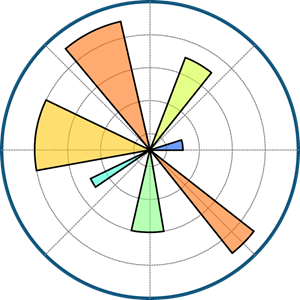
\includegraphics[width=2.5cm]{img/simulation/morphologischer-kasten/simple-gui.png}
        &
        Unreal Engine \newline
        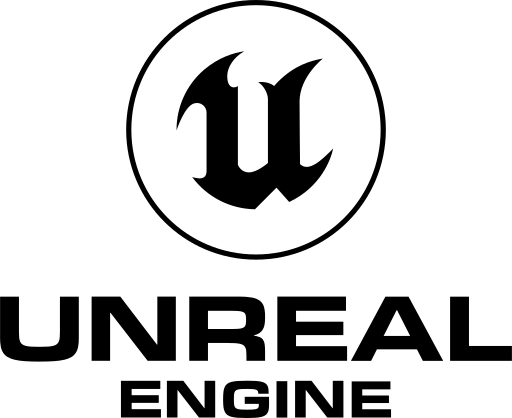
\includegraphics[width=2.5cm]{img/simulation/morphologischer-kasten/unreal-engine-logo.png}
        \\ \hline
        
        \textbf{Wegfindungs-Algorithmus}  &
        \cellcolor{LightGreen}
        Externe Bibliothek &
        Eigene Implementation &
        \\ \hline
        
        \textbf{Programmiersprache}      &
        \cellcolor{LightGreen}
        Python \newline
        
\includegraphics[width=2.5cm]{img/simulation/morphologischer-kasten/python.png} 
        &
        JavaScript \newline
        
\includegraphics[width=2.5cm]{img/simulation/morphologischer-kasten/javascript.png}
        &
        Java \newline
        
\includegraphics[width=2.5cm]{img/simulation/morphologischer-kasten/java.png}
        \\ \hline
        
        \textbf{Informationen \newline einlesen}  &     
        Bilder mit Objekterkennung \newline
        
\includegraphics[width=2.5cm]{img/simulation/morphologischer-kasten/ai-logo.jpg}
        &
        \cellcolor{LightGreen}
        Konfigurationsdatei \newline
        
\includegraphics[width=2.5cm]{img/simulation/morphologischer-kasten/yaml.png}
        &
        \\ \hline
        
        \textbf{Hindernis \newline Bewältigung}   &     
        Immer umfahren \newline
        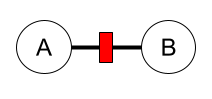
\includegraphics[width=3cm]{img/simulation/morphologischer-kasten/hindernis-umfahren.png}
        &
        Keine spezielle Behandlung \newline
        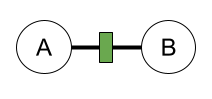
\includegraphics[width=3cm]{img/simulation/morphologischer-kasten/hindernis-ignoriert.png}
        &
        \cellcolor{LightGreen}
        Gewicht hinzufügen\newline
        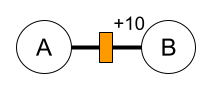
\includegraphics[width=3cm]{img/simulation/morphologischer-kasten/hindernis-gewicht.png}
        \\ \hline
    \end{tabularx}
    \label{tab:sim_Morphologischer_Kasten}
    \caption{Morphologischer Kasten - Simulator}
\end{table}

\paragraph{User Interface}

Obwohl ebenfalls eine virtuelle Umgebung mit der Unreal Engine und dem Pfadfinder-Model existiert, ist der Aufwand zu gross, diese an den Simulator anzubinden. Die Ausgabe in einem Terminal hingegen ist zu minimal. Deshalb wird das User Interface mit einem einfachen GUI umgesetzt. 

\paragraph{Wegfindungs-Algorithmus}

Die Umsetzung des Wegfindungs-Algorithmus kann entweder eigenständig oder mithilfe einer externen Bibliothek erfolgen. Da zahlreiche etablierte Bibliotheken für die Graphentheorie verfügbar sind, erscheint eine eigenständige Implementierung nicht sinnvoll. Dies führt zwar zu einer geringeren Flexibilität, reduziert jedoch die Fehleranfälligkeit erheblich.

\paragraph{Programmiersprache}

Für die Wahl der Programmiersprache wurden Python, JavaScript und Java in Betracht gezogen. Java ist im Informatik-Studium weit verbreitet und wird für zahlreiche Projekte eingesetzt. JavaScript bietet die Möglichkeit, grafische Darstellungen unkompliziert über eine Webseite zu realisieren. Python zeichnet sich durch seine einfache Handhabung aus und wird häufig im Bereich der Künstlichen Intelligenz verwendet, was für die Software des autonomen Roboters wichtig ist.

Python wurde als Programmiersprache gewählt, da innerhalb des Teams umfassendes Know-how vorhanden ist. Darüber hinaus stellt die Bibliothek NetworkX\footnote{https://networkx.org} eine leistungsstarke Lösung für die Arbeit mit Graphen bereit, die optimal für die Anforderungen des Projekts geeignet ist.

\paragraph{Informationen einlesen}

Damit die Software die Hindernisse auf dem Graphen kennt, müssen entsprechende Informationen eingelesen werden können. Idealerweise erfolgt dies ähnlich wie in der Realität, durch die Auswertung von Bildern mittels Objekterkennung. Um den Simulator jedoch möglichst schnell einsatzfähig zu machen, wird stattdessen eine Konfigurationsdatei verwendet, die die notwendigen Informationen bereitstellt.

Die Konfigurationsdatei ermöglicht eine einfache Anpassung der Szenarien und erlaubt dadurch das effiziente Testen verschiedener Konstellationen. Diese Herangehensweise beschleunigt die Entwicklungsphase und sorgt für Flexibilität beim Simulieren diverser Bedingungen.

\paragraph{Hindernis Bewältigung}

Der Simulator soll aufzeigen, wie Hindernisse auf der Strecke behandelt werden.
Dabei wird berücksichtigt, dass Hindernisse unter bestimmten Bedingungen nicht immer umfahren werden können, beispielsweise wenn sämtliche alternativen Wege blockiert sind. Daher stellt die Option `Immer umfahren` keine sinnvolle Strategie dar.

Das Ignorieren von Hindernissen ist ebenfalls suboptimal, da gleich lange Pfade ohne Hindernisse effizienter befahren werden können. Um diesem Problem zu begegnen, wird die Strategie `Gewicht hinzufügen` angewendet. Mit dieser Methode kann flexibel entschieden werden, wie stark ein Hindernis die Wahl eines Pfades beeinflusst. Die Gewichtung erlaubt es, Hindernisse dynamisch in die Berechnung einzubeziehen, ohne zwingend alle Alternativen auszuschliessen.

\subsubsection{Konzept}

Im Optimalfall würde der Simulator die gesamte Hardware des autonomen Fahrzeugs nachbilden. Dadurch könnte die Fahrzeugsoftware direkt im Simulator getestet werden, ohne Anpassungen vornehmen zu müssen. Diese Herangehensweise würde eine nahtlose Integration zwischen Softwareentwicklung und Simulation ermöglichen. Allerdings ist die vollständige Simulation der Hardware mit erheblichem Aufwand verbunden und übersteigt den Rahmen des Simulators.

Der Simulator wird so konzipiert, dass er anhand einer vorgegebenen Konfiguration den optimalen Weg zum Ziel findet. Diese Konfiguration beinhaltet:
\begin{itemize}
    \item Das Ziel: A, B oder C.
    \item Die Strafe (Gewichtung) für das Befahren von Linien mit einem Hindernis.
    \item Objekte die dem Simulator freigegeben werden, sobald sie im Blinkwinkel der Kamera ersichtlich sind:
     \begin{itemize}
        \item Wegpunkte mit einem Pylon 
        \item Entfernte Linien
        \item Erkannte Hindernisse
   \end{itemize}
   \item Objekte (gleich wie oben) diInformationene nicht von der Kamera, sondern erst von der Hardware beim Befahren erkannt werden.
\end{itemize}

Die Informationen, die nicht von der Kamera erkannt werden können, simulieren die realistische Möglichkeit, dass nicht alle Objekte von der Objekterkennung erkannt werden.  

Damit die Simulation weiss, auf welchen Wegpunkten bzw. Linien sich Hindernisse befinden, wird jeder Wegpunkt beschriftet:

\imagewidth{img/simulation/labeled-graph.png}{Beschrifteter Graph}{10cm}


\subsection{Umsetzung}
TODO(Gian): Kapitel vervollständigen

\subsubsection{Konfiguration} \label{sim:Konfiguration}

Die Konfiguration wird in einer \acrshort{yaml}-Datei abgespeichert und sieht wie folgt aus.

\begin{minted}[fontsize=\small]{yaml}
end: B
weight: 3
detectable:
  cones: [E]
  obstacles: 
    - [S, F]
    - [F, A]
  removed:
    - [D, B]
    - [G, C]
undetectable:
  removed:
    - [D, C]
\end{minted}

In der Beispielkonfiguration wird das Ziel \textbf{B} definiert. Hindernisse auf Linien erhalten eine \textbf{dreifache Gewichtung} im Vergleich zu normalen Linien. 

\paragraph{Erklärung Ablauf durch Beispielkonfiguration}

In diesem Abschnitt wird der Ablauf wird anhand der Beispielkonfiguration in Kapitel \ref{sim:Konfiguration} genauer erklärt.

Zu Beginn der Simulation hat der Simulator noch keine Informationen und berechnet den schnellsten Weg von S nach B: \textit{[S, E, A, B]}. Das Fahrzeug dreht sich somit zum nächsten Knoten \textit{E}.

Um zu überprüfen, ob sich Objekte auf der idealen Strecke befindet, schiesst die Kamera ein Bild. In dem Kamerafeld (120° Winkel) sind auf der aktuellen Position \textit{S} mit dem Winkel richtung Wegpunkt \textit{E} folgende Objekte erkennbar:
\begin{itemize}
    \item Auf dem \textbf{Knoten E} befindet sich eine Pylone.
    \item Auf der \textbf{Kante S-F} befindet sich ein Hindernis.
    \item Auf der \textbf{Kante F-A} befindet sich ein Hindernis.
\end{itemize}

Anhand von diesen Informationen wird der schnellste Weg neu berechnet: \textit{[S, G, D, B]}.
Das Fahrzeug dreht richtung Wegpunkt \textit{G}, die Kamera schiesst ein Bild und erhält neue Informationen:
\begin{itemize}
    \item Die \textbf{Kante G-C} ist nicht vorhanden.
\end{itemize}

Nach Einbezug der neu erhaltenen Informationen bleibt der schnellste Weg unverändert.
Deshalb fährt das Fahrzeug nun von Wegpunkt \textit{S} zu \textit{G} und der Ablauf beginnt von vorne:

\begin{itemize}
    \item Das Fahrzeug dreht sich zu Wegpunkt \textit{D} und entdeckt neue Informationen:
    \begin{itemize}
        \item Die \textbf{Kante D-B} ist nicht vorhanden.
    \end{itemize}
    \item Es wird ein neuer Weg berechnet, wobei der Wegpunkt \textit{D} als nächste Option gleich bleibt: \textit{[G, D, C, B]}. Somit wird der Wegpunkt \textit{D} befahren.
    \item Das Fahrzeug dreht sich zu Wegpunkt \textit{C} und entdeckt keine neue Informationen.
    \item Das Fahrzeug versucht loszufahren, aber die Sensoren finden die Linie \textit{[D, C]} nicht.
    \item Die entfernte Linie \textit{[D, C]} wird zum Graphen hinzugefügt und der schnellste Weg neu berechnet: \textit{[D, A, B]}
    \item Das Fahrzeug dreht sich zu Wegpunkt \textit{A} und entdeckt keine neue Informationen.
    \item Das Fahrzeug fährt zu Wegpunkt \textit{A}.
    \item Das Fahrzeug dreht sich zu Wegpunkt \textit{B} und entdeckt keine neue Informationen.
    \item Das Fahrzeug fährt zu Wegpunkt \textit{B}.
    \item Das Fahrzeug befindet sich auf dem Ziel, wodurch ein Zielsignal aufleuchetet.
\end{itemize}



Diese Informationen werden genutzt, um den Graphen dynamisch zu aktualisieren und die optimalen Routen basierend auf den aktuellen Bedingungen neu zu berechnen.


\subsubsection{Ablauf}
In der Abbildung \ref{fig:img/simulation/Simulator_Laufzeitdiagramm.png} ist ein Laufzeitdiagramm des Simulators abgebildet. Darauf werden die wichtigsten Abläufe des Simulators aufgezeigt. 

\imagewidth{img/simulation/Simulator_Laufzeitdiagramm.png}{Simulator Laufzeitdiagramm}{\textwidth}

Der Simulator 
\imagewidth{img/simulation/simulator.png}{Simulator in Aktion}{10cm}


Verwendete Bibliotheken:

\begin{itemize}
    \item NetworkX
    \item Matplotlib
\end{itemize}

\end{document}